%%%%%%%%%%%%%%%%%%%%%%%%%%%%%%%%%%%%%%%%%%%%%%%%%%%%%%%%%%%%%%%%%%%%%%%%%
% Antes de correr el código:
% 1. Ingresar al Menu
% 2. Cambiar la opción "Compiler" a XeLaTeX
% 3. Cambiar la opción "TeX live version" a 2020 (opacidad de la imagen)
%%%%%%%%%%%%%%%%%%%%%%%%%%%%%%%%%%%%%%%%%%%%%%%%%%%%%%%%%%%%%%%%%%%%%%%%%
\documentclass[10pt]{article}
\usepackage[T1]{fontenc}
\usepackage[utf8]{inputenc}
\usepackage[english]{babel}
\usepackage{listings}
\lstset{language=R}
\usepackage[a4paper]{geometry}
\usepackage[dvipsnames]{xcolor}
\usepackage[framemethod=TikZ]{mdframed}
\usepackage{graphicx,tikz}
\usepackage{array}
\usepackage{float}
\usepackage{tocloft}
\setlength{\cftsecnumwidth}{2em}

\geometry{top=2.54cm, bottom=2.54cm, left=2.54cm, right=2.54cm}

\usepackage{url}
\usepackage{lipsum} 
\usepackage{wrapfig}
\usepackage{subcaption}
\usepackage{multicol}

%==========================================
%======     FUENTE PARA CÓDIGOS      ======
%==========================================
\definecolor{codegreen}{rgb}{0,0.6,0}
\definecolor{codegray}{rgb}{0.1,0.1,0.1}
\definecolor{backcolour}{rgb}{0.98,0.98,0.98}

\lstdefinestyle{mystyle}{
  backgroundcolor=\color{backcolour},   
  commentstyle=\color{codegreen},
  keywordstyle=\color{blue},
  numberstyle=\tiny\color{codegray},
  stringstyle=\color{codegreen},
  basicstyle=\ttfamily\footnotesize,
  breakatwhitespace=false,         
  breaklines=true,                 
  captionpos=b,                    
  keepspaces=true,                 
  numbers=left,                    
  numbersep=5pt,                  
  showspaces=false,                
  showstringspaces=false,
  showtabs=false,                  
  tabsize=2
}

%==========================================
%==========     ESTILO TITLE     ==========
%==========================================
\newcommand{\City}[1]{\def\City{#1}}

\makeatletter         
\renewcommand\maketitle{
\begin{flushleft}
{\textcolor{black}{\huge \bfseries \@title }}\\[1ex]
\rule{\textwidth}{0.6pt}\\
\end{flushleft}
\vspace{-0.5cm}

\begin{flushleft}
\textcolor{black}{{\large  \@author} }\\[2ex]
\end{flushleft} } % Note the extra }
\makeatother

%==========================================
%==========    ESTILO CAPTION    ==========
%==========================================
\usepackage{caption}
\captionsetup[table]{name=Tabla ,textfont={it}, labelfont={bf},
                     justification=centering,
                     width =\dimexpr \textwidth-0.5cm\relax}
\captionsetup[figure]{textfont={it}, labelfont={bf},
                      justification=centering, skip=2pt,
                      belowskip=-5pt}
                      
%==========================================
%==========     ESTILO ITEM      ==========
%==========================================
\renewcommand{\labelitemi}{$\bullet$} 
\renewcommand{\labelitemii}{$\circ$} 
\renewcommand{\labelitemiii}{$\cdot$} 

%==========================================
%===    LINKS (Agregar Hyperlinks)     ====
%==========================================
\usepackage[style=apa,
            urldate=long]{biblatex} 
\addbibresource{Bib.bib}

\DeclareSourcemap{
  \maps[datatype=bibtex]{
    \map{
      \step[fieldsource=note, final]
      \step[fieldset=addendum, origfieldval, final]
      \step[fieldset=note, null]}
      }
}

\DefineBibliographyStrings{english}{urlseen = {Accessed }    
}

\usepackage[colorlinks=true,linkcolor=RoyalBlue,
            citecolor=RoyalBlue,urlcolor=RoyalBlue]{hyperref}

%==============================================================
%==============================================================
\title{ }

%%%%%%%%%%%%%%%%%%%%%%%%%%%%%%%%%%%%%%%%%%%%%%%%%%%%%%%%%%%%%%%
%%%%%%%%%%%%                 INICIO                %%%%%%%%%%%% 
%%%%%%%%%%%%%%%%%%%%%%%%%%%%%%%%%%%%%%%%%%%%%%%%%%%%%%%%%%%%%%%
\begin{document}

\begingroup
\let\clearpage\relax % prevent extra page breaks
\thispagestyle{empty}
\begin{center}
{\huge \bfseries Universidad de los Andes}

\vspace{25pt}
{\LARGE \bfseries Departamento de Ingeniería de Sistemas}

\vspace{15pt}

\includegraphics[width=100pt]{images/logo.png} 

\vspace{35pt}
{\LARGE \bfseries Laboratorio \#2: Análisis De Protocolos De La Capa De Aplicación}
\vspace{55pt}

{\Large \bfseries ISIS3204 - Infraestructura de Comunicaciones}


\vspace{100pt}
{\Large \bfseries Grupo 3: }

\end{center}

\begin{flushleft}
  \setlength{\parskip}{0pt}
  \setlength{\itemsep}{0pt}
  \hspace*{4cm}\large\bfseries Juan Esteban Quiroga - 202013216

  \hspace*{4cm}\large\bfseries Juan Manuel Rodriguez - 202013372

  \hspace*{4cm}\large\bfseries Andres Felipe Ortiz - 201727662
\end{flushleft}

\begin{center}
\vspace{60pt}

\Large\bfseries 2025-10
\end{center}

\mbox{}
\endgroup

\clearpage

\tableofcontents
\clearpage


\renewcommand{\thesection}{\arabic{section}}
\section*{Introducción}
\addcontentsline{toc}{section}{Introducción}
Lorem ipsum dolor sit amet, consectetur adipiscing elit. Sed nec tristique eros. Vestibulum ante ipsum primis in faucibus orci luctus et ultrices posuere cubilia curae; Pellentesque sit amet purus a sapien porta viverra. Cras in feugiat nisl. Mauris volutpat lorem in ligula dapibus, non aliquam eros tristique. Suspendisse potenti. Nunc laoreet augue ac viverra dictum. Integer mattis magna in nisi consequat, nec vehicula nulla dignissim. Ut nec aliquam libero. Sed eu nisl vitae mauris congue eleifend at nec urna.

%==============================================================
%=====================   8.1   ================================
%==============================================================
\renewcommand{\thesection}{8.\arabic{section}}
\setcounter{section}{0}
\section{Prueba ping}

Lorem ipsum dolor sit amet, consectetur adipiscing elit. Sed nec tristique eros. Vestibulum ante ipsum primis in faucibus orci luctus et ultrices posuere cubilia curae; Pellentesque sit amet purus a sapien porta viverra.


\begin{figure}[H]
    \centering
    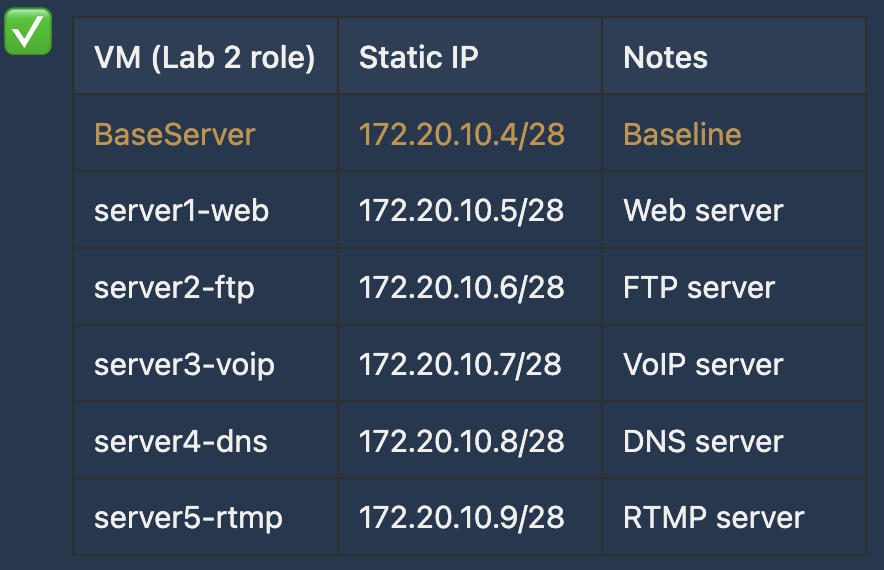
\includegraphics[width=0.65\textwidth]{lab-02-screenshots/server-ips.png}
    \caption{Configuración de IPs estáticas}
\end{figure}


\subsection{Prueba de conectividad al servidor DNS}
\subsection{Prueba de conectividad al servidor FTP}


%==============================================================
%=====================   8.2   ================================
%==============================================================
\renewcommand{\thesection}{8.\arabic{section}}
\section{Análisis de tráfico del Servicio DNS}
\subsection{Prueba de conectividad al Servidor Web (IP)}
\subsection{Prueba de conectividad al Servidor Web (URL)}


%==============================================================
%=====================   8.3   ================================
%==============================================================
\renewcommand{\thesection}{8.\arabic{section}}
\section{Análisis de tráfico del Servicio FTP}
\subsection{Conexión al servidor FTP}
\subsection{Descarga de archivo (Download)}
\subsection{Carga de archivo (Upload)}

%==============================================================
%=====================   8.4   ================================
%==============================================================
\renewcommand{\thesection}{8.\arabic{section}}
\section{Análisis de tráfico del Servicio Web}
\subsection{Acceso al servidor web mediante HTTP}

%==============================================================
%=====================   8.5   ================================
%==============================================================
\renewcommand{\thesection}{8.\arabic{section}}
\section{Análisis del protocolo HTTPS realizando navegación en el sitio de YouTube}

\subsection{Navegación en YouTube}
Se realizó la captura de tráfico mientras se navegaba en el sitio \textbf{https://www.youtube.com/}. 
Para reducir interferencias, se mantuvo una única pestaña activa en el navegador. 
Además, se inició sesión con una cuenta de Gmail y se realizaron acciones como la visualización de videos y la publicación de comentarios. 
La captura se guardó con el nombre \texttt{YouTube\_view.pcapng}.

\begin{itemize}
    \item \textbf{Filtro aplicado:} \texttt{tcp.port == 443}
    \item \textbf{Capa de aplicación:} Se identificaron protocolos TLS 1.2 y TLS 1.3 con mensajes como \textit{Client Hello}, \textit{Server Hello}, \textit{Certificate} y \textit{Application Data}. Estos forman parte del \textit{handshake TLS} y del intercambio de datos cifrados.
    \item \textbf{Capa de transporte:} Se utilizó el protocolo \textbf{TCP}, que asegura confiabilidad en la comunicación.
    \item \textbf{Puertos:} El puerto destino fue el estándar \textbf{443 (HTTPS)} y los puertos de origen fueron dinámicos (efímeros), variando en cada sesión.
    \item \textbf{Servidores (SNI):} Se evidenciaron dominios de Google asociados a YouTube como \texttt{youtube.com}, \texttt{googlevideo.com} y \texttt{ytimg.com}.
\end{itemize}

\noindent
\textbf{Conclusiones:} Todo el tráfico de YouTube viaja cifrado mediante TLS, garantizando la confidencialidad de la comunicación. 
El uso de múltiples dominios de Google refleja la distribución de contenidos (streaming de video, recursos multimedia, etc.). 
El tráfico aparece como \textit{Application Data}, confirmando que no es posible acceder al contenido real debido al cifrado.

%--------------------------------------------------------------

\subsection{Navegación en otros sitios HTTPS}
Se realizó una segunda captura al visitar diferentes portales colombianos y académicos, guardada como \texttt{HTTPS\_view.pcapng}.

\subsubsection{https://www.elespectador.com}
El análisis mostró conexiones TLS (1.2 y 1.3) sobre el puerto 443 utilizando TCP como protocolo de transporte. 
La información de aplicación corresponde a \textit{handshake TLS} y \textit{Application Data}. 
El tráfico se mantiene cifrado en todo momento.

\subsubsection{https://www.eltiempo.com}
Similar a \textit{El Espectador}, se evidenció el uso de TLS sobre TCP, puerto 443. 
Los paquetes de aplicación muestran únicamente intercambio de certificados y datos cifrados. 
El sitio garantiza confidencialidad en la comunicación.

\subsubsection{https://www.uniandes.edu.co}
El portal de la Universidad de los Andes utiliza también HTTPS con TLS 1.2/1.3. 
La captura evidencia el proceso de \textit{handshake TLS} y la posterior transmisión de datos cifrados bajo \textit{Application Data}. 
Esto asegura la protección de información académica y de los usuarios.

\subsubsection{https://www.bancolombia.com}
La conexión al portal bancario utiliza \textbf{TLS 1.3} sobre TCP/443, garantizando un nivel de seguridad reforzado debido a la naturaleza sensible de la información financiera. 
Todos los datos observados corresponden a mensajes TLS cifrados. 
Esto valida que el tráfico cumple con los estándares de seguridad exigidos en el sector bancario.

\noindent
\textbf{Conclusiones generales:} 
En todos los portales analizados, el tráfico de red se ejecuta mediante el protocolo HTTPS sobre TCP/443, con versiones TLS 1.2 y 1.3. 
La capa de aplicación muestra únicamente información relacionada con el protocolo TLS y no expone contenido en claro. 
Esto confirma que los mecanismos de seguridad actuales protegen efectivamente la confidencialidad e integridad de la comunicación entre cliente y servidor.

%==============================================================
%=====================   Flujos   =============================
%==============================================================

\subsection*{Representación gráfica de flujos}

Para complementar el análisis, se generaron diagramas de flujo en Wireshark que muestran la interacción entre el cliente y los servidores durante la navegación. 
Estos flujos permiten observar de manera visual el establecimiento de las conexiones, los intercambios de datos cifrados y los cierres de sesión.

\begin{figure}[H]
    \centering
    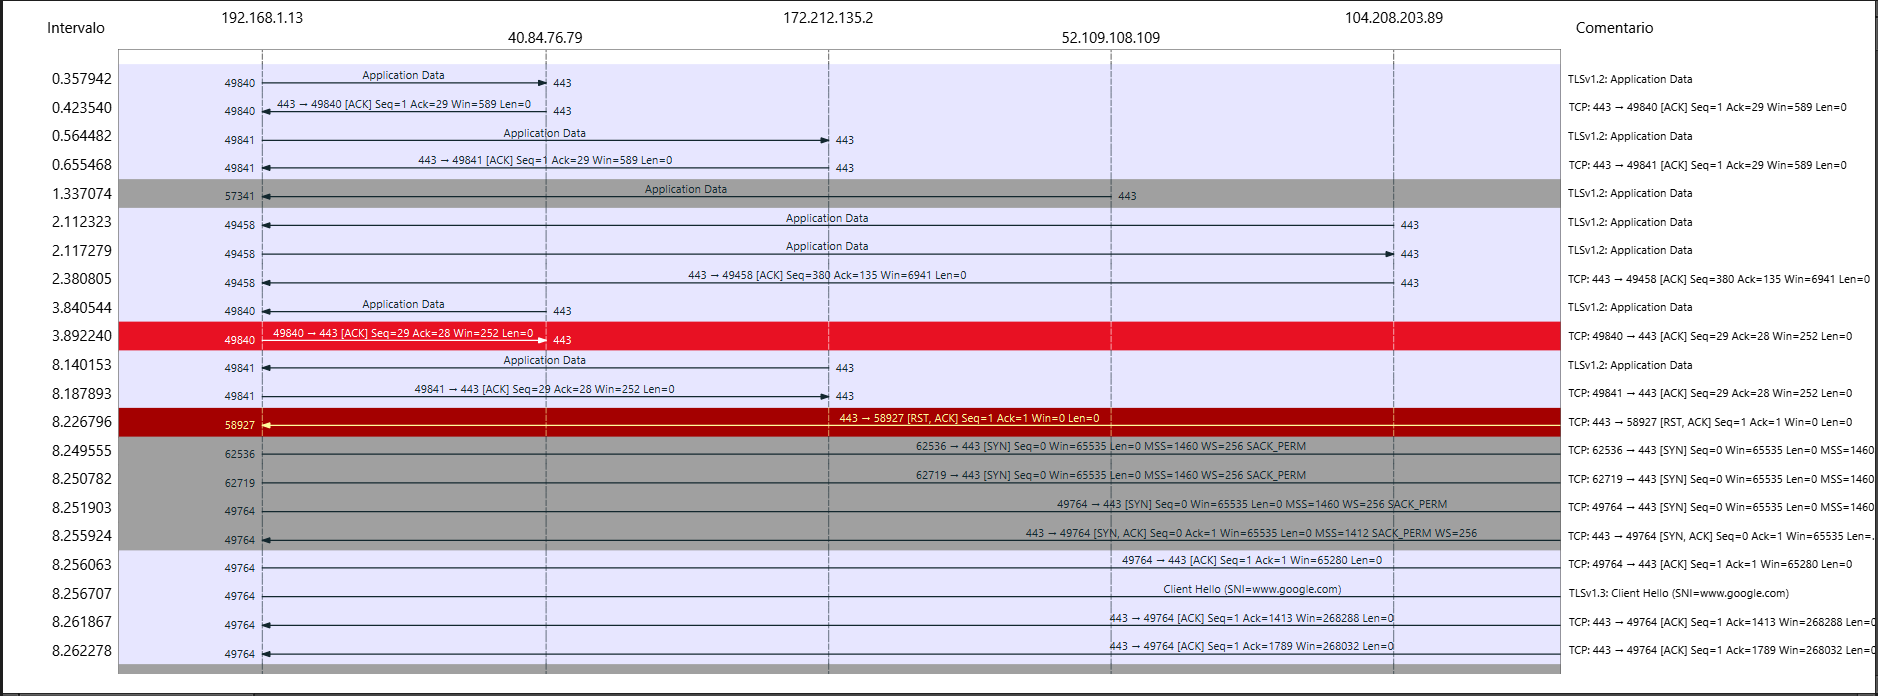
\includegraphics[width=0.95\textwidth]{lab-02-screenshots/8.5-YouTube-flow.png}
    \caption{Flujo de comunicación durante la navegación en YouTube. 
    Se observan múltiples paquetes \texttt{Application Data} correspondientes al tráfico de video en streaming, así como respuestas TCP de control (\texttt{ACK}). 
    El diagrama refleja conexiones hacia diferentes direcciones IP asociadas a servidores de Google y YouTube.}
\end{figure}

\begin{figure}[H]
    \centering
    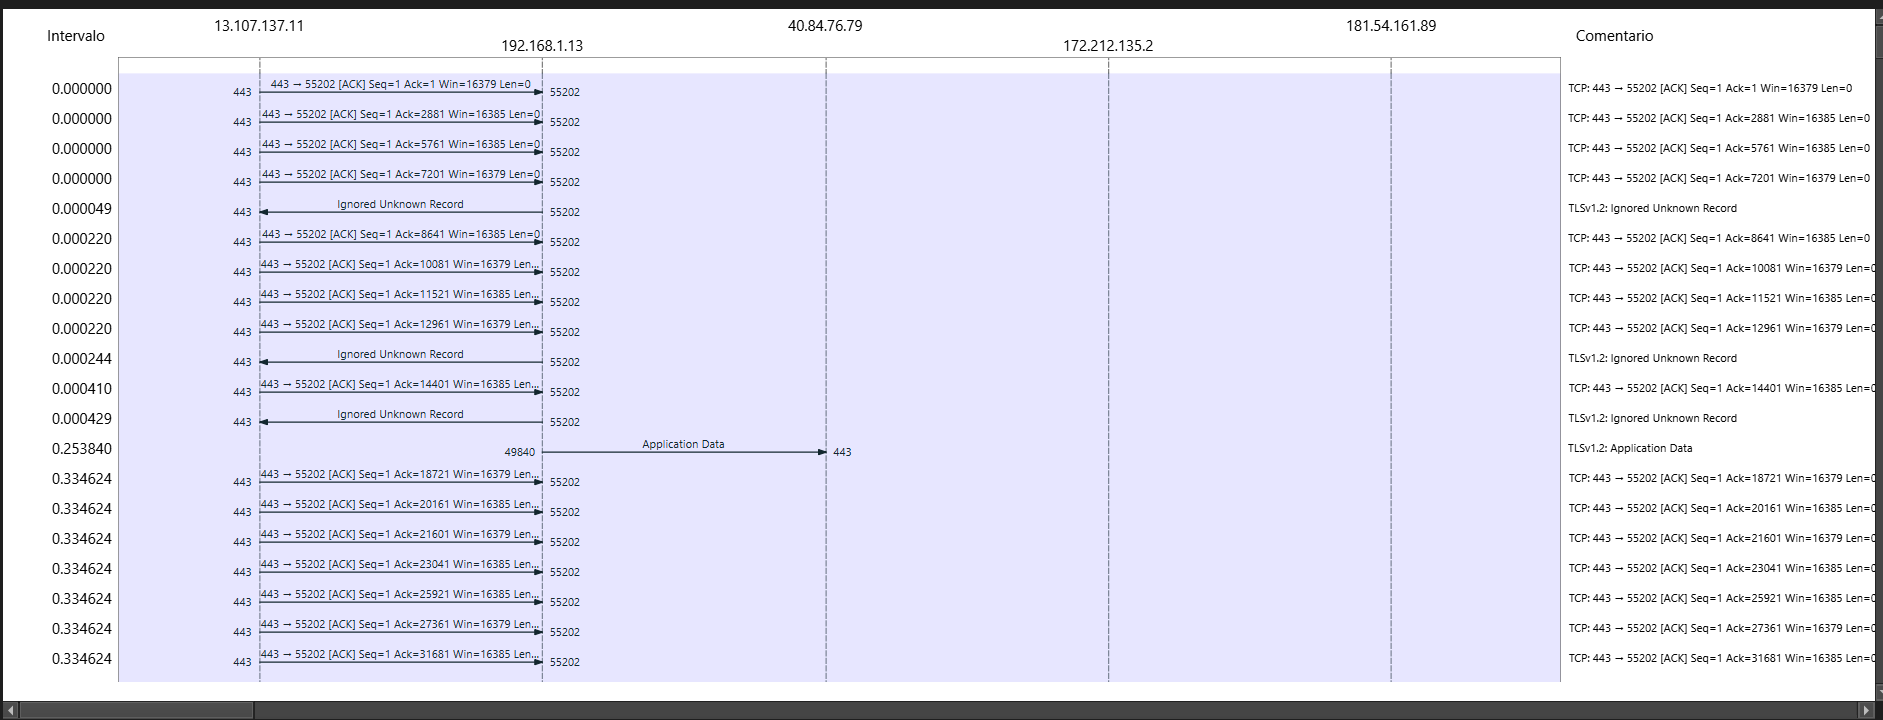
\includegraphics[width=0.95\textwidth]{lab-02-screenshots/8.5-HTTPS-flow.png}
    \caption{Flujo de comunicación durante la navegación en otros sitios HTTPS (El Espectador, El Tiempo, Uniandes y Bancolombia). 
    El diagrama muestra el proceso de establecimiento de conexión (\texttt{SYN}, \texttt{ACK}), seguido del intercambio de datos cifrados mediante TLS 1.2 y 1.3. 
    Destaca la aparición de mensajes \texttt{Client Hello} que evidencian el inicio del \textit{handshake TLS}, así como varios paquetes de \texttt{Application Data} que corresponden a la carga de contenido.}
\end{figure}



%==============================================================
%=====================   8.6  ================================
%==============================================================
\renewcommand{\thesection}{8.\arabic{section}}
\section{Análisis del protocolo VoIP}
\subsection{Establecimiento de la llamada}


%==============================================================
%=====================   8.7   ================================
%==============================================================
\renewcommand{\thesection}{8.\arabic{section}}
\section{Análisis del protocolo RTMP}
\subsection{Inicio de la transmisión}


%==============================================================
%=====================   8.7   ================================
%==============================================================
\renewcommand{\thesection}{9.\arabic{section}}
\setcounter{section}{0}
\section{Topología}












\begin{thebibliography}{9}


  \bibitem{kurose_ross}
  Computer Networking, a top-down approach. James Kurose, Keith Ross. Addison-Wesley, 6th ed.

  \end{thebibliography}


\end{document}